\section{Introduction}

This note describes a study of electroweak (EWK) productions of W+2jets using the CMS detector~\cite{JINST} in pp collisions at $\sqrt{s}=8$\,TeV,  in events with a leptonically decaying W boson  (W$\to\ell\nu$, $\ell=e,\mu$), and also with Vector Boson Fusion (VBF) like requirement
that the weak boson is centrally produced and that the two jets are well separated in rapidity.

VBF has been playing an important role in Higgs discovery and property measurement at
the LHC, which, nevertheless, depends on understanding the detector response and validating the Monte-Calo generator to
a good level of accuracy, including the selection of the forward jets 
and the veto of the additional central jets. Therefore, it is useful to have other promising processes by which to
validate the VBF methodology~\cite{Green:2005zb,Govoni:2010bb}. The EWK production of a Z or W boson with subsequent leptonic
decay appears to be ideal in that there are similar VBF like Feynman diagrams for EWK Z/W as for Higgs
VBF productions. Moreover, as shown in \cite{Oleari:2003tc}, these EWK processes have more sizable cross section than the VBF Higgs channels at the LHC and thus are promising to be measured precisely.

These EWK processes have already been studied in the investigation of rapidity gaps at hadron
colliders~\cite{Rainwater:1996ud,Khoze:2002fa}, as a probe of anomalous triple-gauge-boson (TGC)
couplings~\cite{Baur:1993fv,Eboli:2004gc} or as a background to Higgs boson searches in VBF channels ~\cite{Rainwater:1998kj,Plehn:1999xi,Rainwater:1999sd,Kauer:2000hi}. 

There are three classes of diagrams in the electroweak production of the $\rm W$ and $\rm Z$ bosons with two
jets: bremsstrahlung, VBF processes and multiperipheral diagrams with a large
negative interference among them~\cite{Khoze:2002fa,Oleari:2003tc}.
Figure~\ref{fig:wz_feynman} shows the representative diagrams for EWK $\ell\nu~\rm jj$
production processes. The large negative interference effects among the VBF and non-VBF EWK diagrams
are in fact related to well-known non-abelian gauge cancellations that preserve the scattering unitar-
ity and the electroweak model theory renormalizability~\cite{'tHooft:1972fi}. This situation makes the VBF Z/W
channel more complicated but also more interesting.

The EWK Z+2jets has recently been studied in CMS using 5~fb${}^{-1}$ of data recorded in 2011~\cite{Chatrchyan:2013jya}. In this note, we focus on EWK W+2jets measurement. The sample is dominated by associated EWK or QCD productions of W boson 
with two or more jets, but also contains diboson events with hadronic
W or Z decay to two jets (W/Z$\to jj$), 
and contribution from top pair ($\ttbar\to l\nu jj$), single top ($pp\to tq \to \ell\nu jj$),
and QCD multijet events. We analyze data sample corresponding to an integrated 
luminosity of 19.3~fb${}^{-1}$.


\begin{figure}[h!]{
\centering
\subfigure[Bremsstrahlung]{
    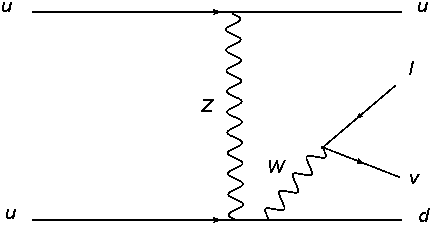
\includegraphics[width=0.31\textwidth]{figs/Diagram1.png}}
\subfigure[VBF]{ 
    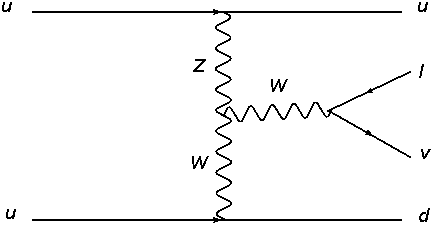
\includegraphics[width=0.31\textwidth]{figs/Diagram2.png}}
\subfigure[Multiperipheral]{ 
    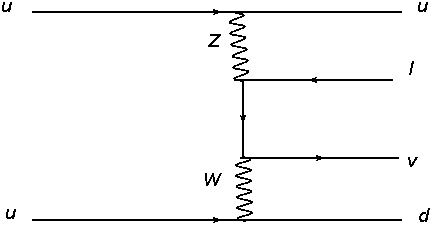
\includegraphics[width=0.31\textwidth]{figs/Diagram3.png}}
\caption{\label{fig:wz_feynman} Representative diagrams for EWK $\ell\nu jj$ productions at the LHC: (a) Bremsstrahlung, (b) VBF, and (c) Multiperipheral processes.}}
\end{figure}
%%%%%%%

%%%%%%%%%%%%%%%
%%%%%%%%%%%%%%%%%
%%\subsection{Connection with Higgs}
%%The Higgs mechanism was conceived to give mass to the $W$ and 
%%$Z$ bosons and break the electroweak gauge symmetry. 
%%The mechanism predicts a Higgs boson particle that interacts with other 
%%particles with a strength proportional to their mass.
%%Since the $W$ and $Z$ bosons are very massive, the Higgs will predominantly 
%%decay to these particles if its mass is at least twice that of the $W$ 
%%or $Z$ boson (see Fig.~\ref{figure:higgs_sm_br}). 
%%Study of boson pair production is thus the first step to Higgs discovery 
%%at the LHC.
%%%%%%%%%
%%\begin{figure}[h!] {\centering
%%    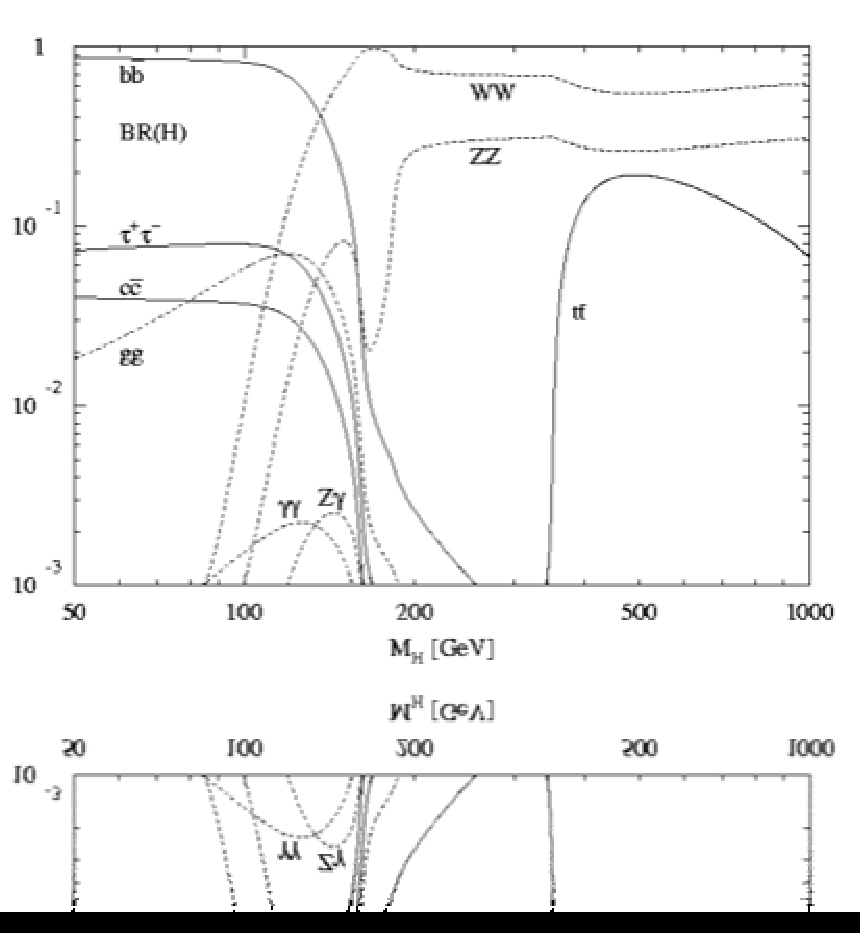
\includegraphics[trim = 0mm 45mm 0mm 0mm, clip, width=0.7\textwidth]{figs/higgs_sm_br.pdf}
%%    \caption{Standard Model Higgs branching fraction as a function of 
%%      Higgs mass}
%%    \label{figure:higgs_sm_br}}
%%\end{figure}
%%%%%%%%%
